\documentclass{elegantbook}
\usepackage[square,numbers,sort&compress]{natbib}
\newcommand{\upcite}[1]{\textsuperscript{\textsuperscript{\cite{#1}}}}
\usepackage{multirow}
\usepackage{color}
\usepackage{tikz}
\usepackage{algorithm}
\usepackage{algorithmic}
\renewcommand{\algorithmicrequire}{ \textbf{Input:}} 
\renewcommand{\algorithmicensure}{ \textbf{Output:}} 
\usetikzlibrary{shapes.geometric, arrows}
\tikzstyle{startstop} = [rectangle, rounded corners, minimum width = 2cm, minimum height=1cm,text centered, draw = black, fill = red!40]
\tikzstyle{acti} = [rectangle, trapezium left angle=70, trapezium right angle=110, minimum width=5cm, minimum height=0.5cm, text centered, draw=black, fill = blue!40]
\tikzstyle{pool} = [rectangle, trapezium left angle=70, trapezium right angle=110, minimum width=2cm, minimum height=0.5cm, text centered, draw=black, fill = purple!40]
\tikzstyle{process} = [rectangle, minimum width=3cm, minimum height=1cm, text centered, draw=black, fill = green!50]
\tikzstyle{conv} = [rectangle, minimum width=3cm, minimum height=1cm, text centered, draw=black, fill = magenta!50]
\tikzstyle{loss} = [rectangle, rounded corners, minimum width = 2cm, minimum height=1cm,text centered, draw = black, fill = yellow!40]
\tikzstyle{arrow} = [->,>=stealth]

% title info
\title{Deep Learning}
\subtitle{MNIST Digits Classification with CNN}
% bio info
\author{Yantian Luo}
\institute{Electronic Engineering}
\version{2018310742}
\date{\today}
\logo{logo.png}
\cover{cover.jpg}

\begin{document}

\maketitle
\tableofcontents
\mainmatter
\hypersetup{pageanchor=true}
% add preface chapter here if needed
\chapter{Introduction}
MNIST digits dataset is a widely used database for image classification in machine learning field. It contains 60,000 training samples and 10,000 testing samples. Each sample is a $784\times1$ column vector, which is transformed from an original $28\times28$ pixels grayscale image.

In this homework, we will continue working on MNIST digits classification problem by utilizing convolutional neural network (CNN). The main challenge is to implement the forward and backpropagation functions of convolutional layer and pooling layer from scratch! And at last, we compare the the difference of results obtained when working with MLP.

\chapter{Algorithm Design}
In this homework, we have basis about the Linear layer, Relu layer, Sigmoid layer, EuclideanLoss and SoftmaxCrossEntropyLoss from homework1, thus we don't need to complete their forward and backward functions another time. Therefore, the most important challenge for us is to implement the forward and backpropagation functions of convolutional layer and
pooling layer.

\section{$im2col$ operation}
This section, we introduce a very important operation for pooling and convolution, that is $im2col$. $im2col$ operation rearranges sliding image neighborhoods of kernel size into columns with padding and stride, and returns the concatenated columns in another tensor. Figure \ref{im2col} shows  an $im2col$ operation on a 2-dimension matrix with kernel-size = (3$\times$3) and padding = 0, stride = 2. From the figure we can find, the column of the output matrix is rearranging sliding image neighborhoods of kernel size. 

\begin{figure}[!ht]
	\centering
	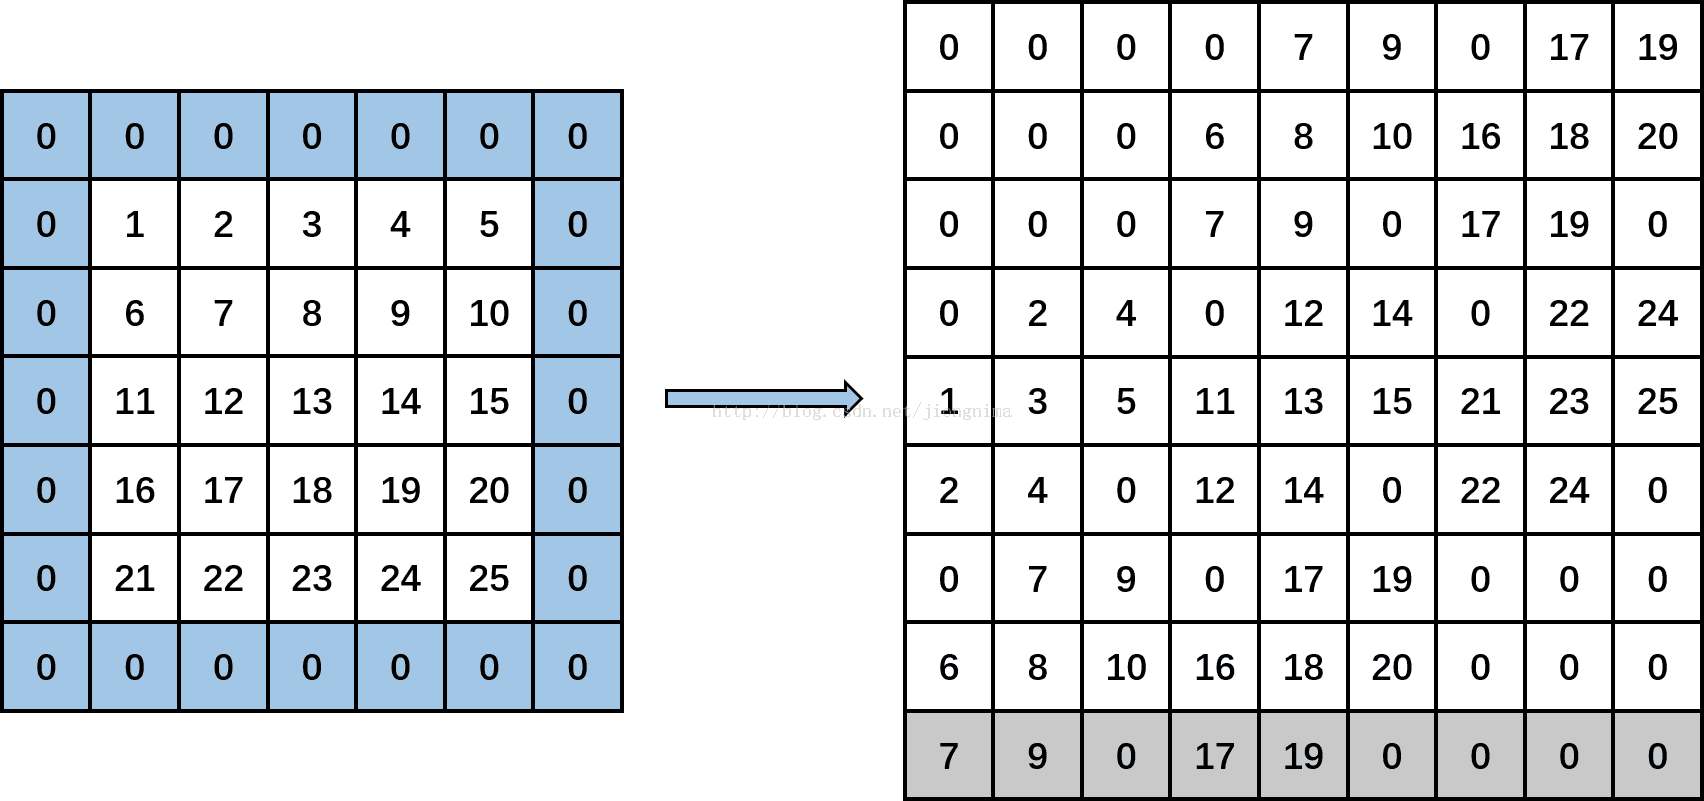
\includegraphics[width=\linewidth]{im2col}
	\caption{\label{im2col}2-dimension $im2col$ operation: left is the input matrix, right is the output matrix with kernel-size = (3$\times$3) and padding = 0, stride = 2}
\end{figure}

%\begin{algorithm}[htb]
%	\caption{$im2col$ operation}
%	\label{alg:im2col}
%	\begin{algorithmic}[1]
%		\REQUIRE input\_tensor=x, kernel size=$h\times w$, padding=p, stride=s
%		\ENSURE output\_tensor=y
%	\end{algorithmic}
%\end{algorithm}

\section{convolution layer}
Using $im2col$ operation, we can easily convert convolution operation to tensor multiplication.

\subsection{Forward}
Assuming the input tensor is $x$ with the shape $n\times c_{in}\times h_{in}\times w_{in}$, the weight matrix is $W$ with the shape $c_{out}\times c_{in}\times k\times k$, the bias is $b$ with the shape $c_{out}$, the kernel\_size is $k$, the pad is $p$ and the output tensor is $y$ with the shape$n\times c_{out}\times h_{out}\times w_{out}$. Using $im2col$ operation we can gey the Forward algorithm as shown in Algorithm \ref{alg:im2col}.

\begin{algorithm}[htb]
	\caption{Convolution Forward Algorithm}
	\label{alg:im2col}
	\begin{algorithmic}[1]
		\REQUIRE $x, W, b, k, p$
		\ENSURE $y$
		\STATE $h_{out}=h_{in}+2\times p-k+1$
		\STATE $w_{out}=w_{in}+2\times p-k+1$
		\STATE $x_t=im2col(x)$ and reshape $x_t^T$ into $x_m$ with shape $h_{out}\times w_{out}\times n\times (c_{in}\times k\times k)$
		\STATE Reshape $W$ with shape $c_{out} \times (c_{in}\times k\times k)$
		\STATE Compute $y=x_m\cdot W^T$
		\STATE At last, transpose $y$ into right shape which is $n\times c_{out}\times h_{out}\times w_{out}$
	\end{algorithmic}
\end{algorithm}

\subsection{Backward}
From the ppt of the class, we can get the gradient and local sensitivity as follow:
\begin{equation}
\begin{aligned}
&\frac{\partial E^{(n)}}{\partial W_q^{(l)}}=Y^{(l-1)}*_{valid} rot180(\delta_q^{(l)}) \\
&\frac{\partial E^{(n)}}{\partial b^{(l)}}=\sum_{i,j}\delta_{ij}^{(l)} \\
&\delta_p^{(l-1)}=\bigtriangleup_q^{(l)}*_{full} flip_0(\tilde{W}_p^{(l)})
\end{aligned}
\end{equation}

From the equation, we can find that the the gradient of $W$ and local sensitivity is also convolution operation, which can be used Algorithm \ref{alg:im2col} to solve it. The radient of $b$ is simply add operation which is easy to implement.
\section{average pooling layer}

\subsection{Forward}
For average pooling layer, we can regard it as convolution layer with $W$ is in equation (\ref{eq1}) and $b=0, pad, stride=k$, then we can also use Algorithm \ref{alg:im2col} to implement Average pooling layer forward operation.
\begin{equation}
\label{eq1}
W=\left[\frac{1}{k\times k}\right]_{c_{in}\times c_{in}\times k\times k}
\end{equation}

\subsection{Backward}
As stated in the course ppt, the backward of average pooling layer satifies equation (\ref{eq2}).
\begin{equation}
\label{eq2}
\delta^{(l-1)}=\frac{1}{poolingsize}upsample(\delta^{(l)})
\end{equation}

The $upsample$ operation can be defined as equation (\ref{eq3})
\begin{equation}
\label{eq3}
upsample(\mathbf{a})\overset{\bigtriangleup}{=}
\left[
\begin{array}{cc|c|cc}
a_{11} & a_{11} & \cdots & a_{1m} & a_{1m} \\
a_{11} & a_{11} & \cdots & a_{1m} & a_{1m} \\
\hline
\vdots & \vdots & \vdots & \vdots & \vdots \\
\hline
a_{n1} & a_{n1} & \cdots & a_{nm} & a_{nm} \\
a_{n1} & a_{n1} & \cdots & a_{nm} & a_{nm}
\end{array}
\right]
\end{equation}
\chapter{Experients and Results}

In this chapter, we use CNN to work on MNIST digits classification problem and get the accuracy and loss, and we compare the difference of results obtained when working
with MLP in homework1. And at last, we visualize the first convolution layer's output after ReLU for 0-9 digit images.

\section{Experiments1 (two conv layers + one linear layer)}
The network structure in this section is designed as Figure \ref{fig1} and training arguments is as follow:

\begin{lstlisting}[frame=single,language=python]  
config = {
	'learning_rate': 0.01,
	'weight_decay': 0.0001,
	'momentum': 0.9,
	'batch_size': 100,
	'max_epoch': 100,
	'disp_freq': 50,
}
\end{lstlisting}

\begin{figure}[htbp]
	\centering
	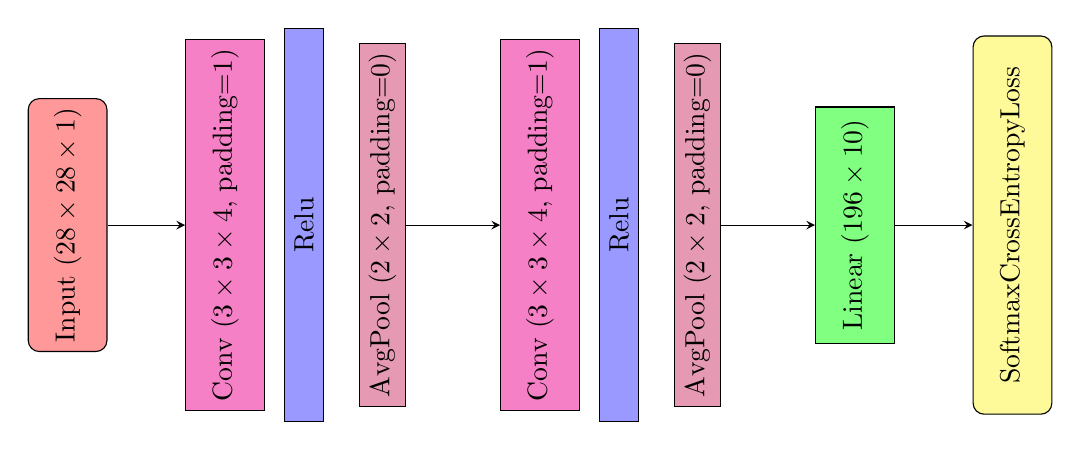
\begin{tikzpicture}
		\node (start) [startstop, rotate=90] {Input ($28\times28\times 1$)};
		\node (conv1) [conv, rotate=90, below of=start, yshift=-1cm] {Conv ($3\times3\times 4$, padding=1)};
		\node (acti1) [acti, rotate=90, below of=conv1] {Relu};
		\node (pool1) [pool, rotate=90, below of=acti1] {AvgPool ($2\times2$, padding=0)};
		\node (conv2) [conv, rotate=90, below of=pool1, yshift=-1cm] {Conv ($3\times3\times 4$, padding=1)};
		\node (acti2) [acti, rotate=90, below of=conv2] {Relu};
		\node (pool2) [pool, rotate=90, below of=acti2] {AvgPool ($2\times2$, padding=0)};
		\node (linear) [process, rotate=90, below of=pool2, yshift=-1cm] {Linear ($196\times10$)};
		\node (loss) [loss, rotate=90, below of=linear, yshift=-1cm, text width=13em] {SoftmaxCrossEntropyLoss};
		
		\draw [arrow](start) -- (conv1);
%		\draw [arrow](conv1) -- (acti1);
%		\draw [arrow](acti1) -- (pool1);
		\draw [arrow](pool1) -- (conv2);
%		\draw [arrow](conv2) -- (acti2);
%		\draw [arrow](acti2) -- (pool2);
		\draw [arrow](pool2) -- (linear);
		\draw [arrow](linear) -- (loss);
	\end{tikzpicture}
	\caption{\label{fig1}Experiments1 Network Structure}
\end{figure}

In this experiments, the accuracy on test set is 0.983 and the loss on test set is 0.052. We draw the train accuracy curve and train loss curve as shown in Figure \ref{trainres1} and we draw the test accuracy curve and test loss curve with respect to epoch as shown in Figure \ref{testres1}

\begin{figure}[!h]
	\centering
	\begin{minipage}[t]{0.48\textwidth}
		\centering
		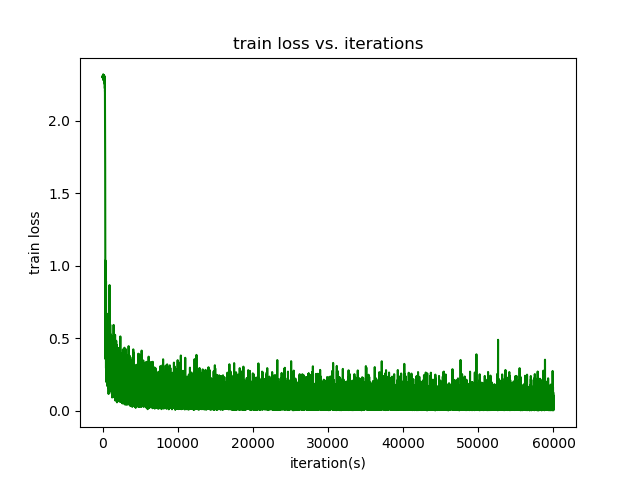
\includegraphics[width=\textwidth]{../results/trainloss1}
	\end{minipage}
	\begin{minipage}[t]{0.48\textwidth}
		\centering
		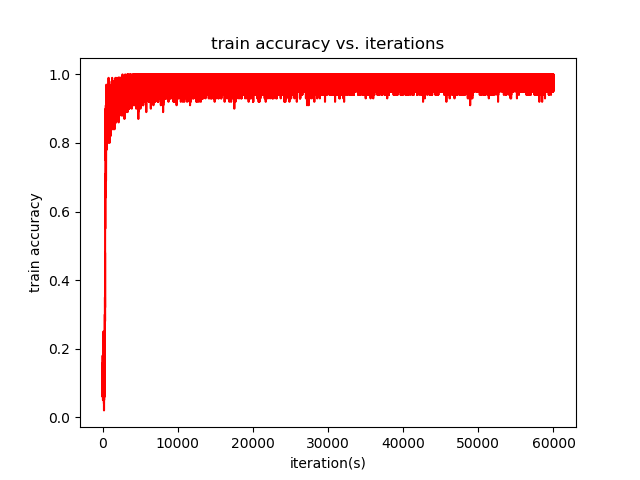
\includegraphics[width=\textwidth]{../results/trainacc1}
	\end{minipage}
	\caption{\label{trainres1}train loss curve and train accuracy curve in Experiments1}
\end{figure}

\begin{figure}[!h]
	\centering
	\begin{minipage}[t]{0.48\textwidth}
		\centering
		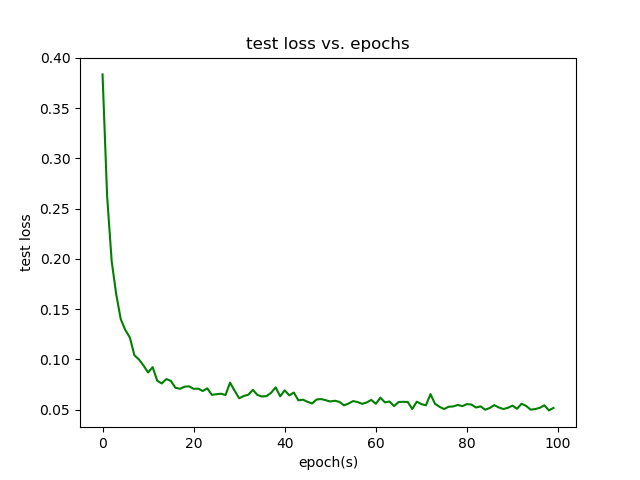
\includegraphics[width=\textwidth]{../results/testloss1}
	\end{minipage}
	\begin{minipage}[t]{0.48\textwidth}
		\centering
		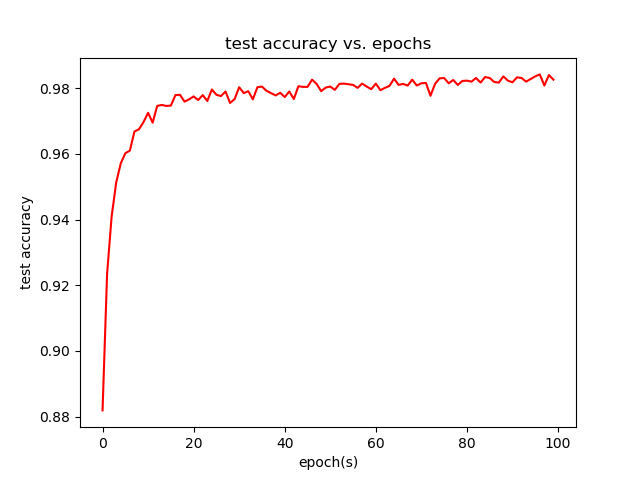
\includegraphics[width=\textwidth]{../results/testacc1}
	\end{minipage}
	\caption{\label{testres1}test loss curve and test accuracy curve in Experiments1}
\end{figure}
%\begin{table}[!ht]
%	\centering
%	\caption{\label{tab1}Network Structure with one hidden layer}
%	\begin{tabular}{|c|c|c|c|c|c|}
%		\hline
%		layer name & Input & Linear & Activation & Linear & Loss \\
%		\hline
%		\multirow{2}{*}{Size} & \multirow{2}{*}{$784 \times 1$} & \multirow{2}{*}{$784 \times 128$} & Relu & \multirow{2}{*}{$128\times 10$} &  EuclideanLoss \\
%		 & & & Sigmoid & &SoftmaxCrossEntropyLoss \\
%		\hline
%	\end{tabular}
%\end{table}



\section{Experiments2 (two conv layers + two linear layers)}
The network structure in this section is designed as Table\ref{tab2} and training arguments is as follow:

\begin{lstlisting}[frame=single,language=python]  
config = {
    'learning_rate': 0.1,
    'weight_decay': 0.0001,
    'momentum': 0.9,
    'batch_size': 100,
    'max_epoch': 100,
    'disp_freq': 50,
}
\end{lstlisting}

\begin{figure}[htbp]
	\centering
	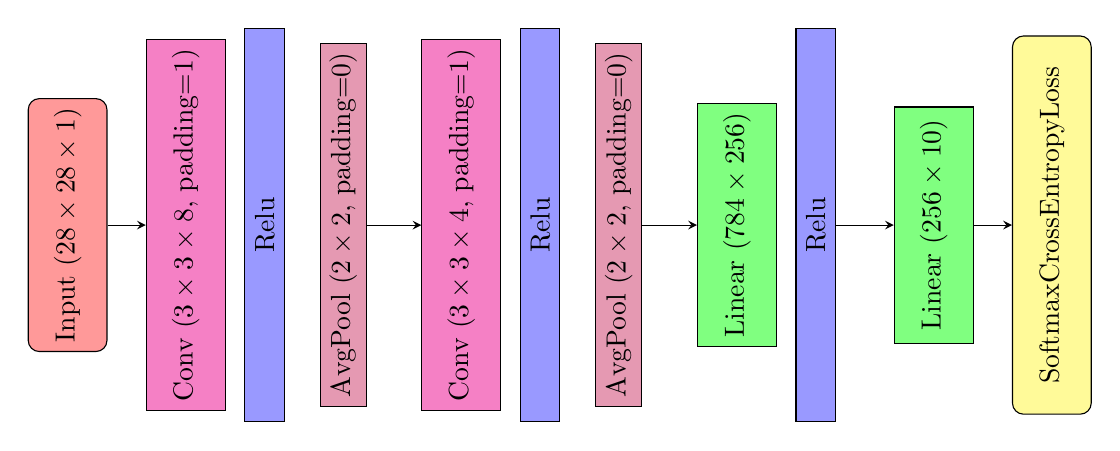
\begin{tikzpicture}
	\node (start) [startstop, rotate=90] {Input ($28\times28\times 1$)};
	\node (conv1) [conv, rotate=90, below of=start, yshift=-0.5cm] {Conv ($3\times3\times 8$, padding=1)};
	\node (acti1) [acti, rotate=90, below of=conv1] {Relu};
	\node (pool1) [pool, rotate=90, below of=acti1] {AvgPool ($2\times2$, padding=0)};
	\node (conv2) [conv, rotate=90, below of=pool1, yshift=-0.5cm] {Conv ($3\times3\times 4$, padding=1)};
	\node (acti2) [acti, rotate=90, below of=conv2] {Relu};
	\node (pool2) [pool, rotate=90, below of=acti2] {AvgPool ($2\times2$, padding=0)};
	\node (linear1) [process, rotate=90, below of=pool2, yshift=-0.5cm] {Linear ($784\times256$)};
	\node (acti3) [acti, rotate=90, below of=linear1] {Relu};
	\node (linear2) [process, rotate=90, below of=acti3, yshift=-0.5cm] {Linear ($256\times10$)};
	\node (loss) [loss, rotate=90, below of=linear2, yshift=-0.5cm, text width=13em] {SoftmaxCrossEntropyLoss};
	
	\draw [arrow](start) -- (conv1);
	%		\draw [arrow](conv1) -- (acti1);
	%		\draw [arrow](acti1) -- (pool1);
	\draw [arrow](pool1) -- (conv2);
	%		\draw [arrow](conv2) -- (acti2);
	%		\draw [arrow](acti2) -- (pool2);
	\draw [arrow](pool2) -- (linear1);
	\draw [arrow](acti3) -- (linear2);
	\draw [arrow](linear2) -- (loss);
	\end{tikzpicture}
	\caption{\label{fig2}Experiments2 Network Structure}
\end{figure}

In this experiments, the accuracy on test set is up to 0.987 and the loss on test set is 0.048 after only 30 training epochs. Then we draw the train accuracy curve and train loss curve as shown in Figure \ref{trainres2} and we draw the test accuracy curve and test loss curve with respect to epoch as shown in Figure \ref{testres2}

\begin{figure}[!h]
	\centering
	\begin{minipage}[t]{0.48\textwidth}
		\centering
		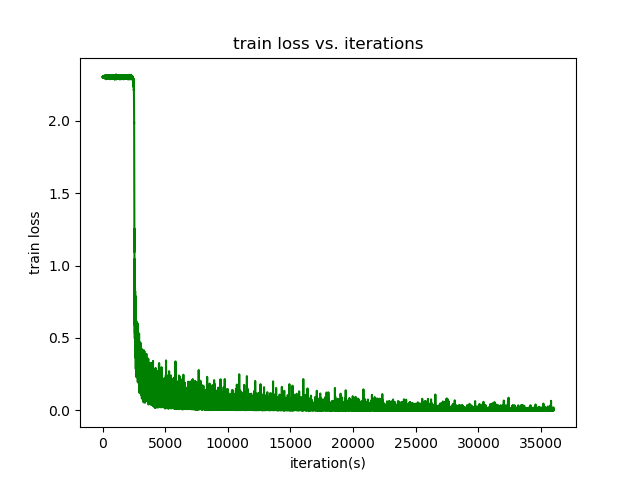
\includegraphics[width=\textwidth]{../results/trainloss2}
	\end{minipage}
	\begin{minipage}[t]{0.48\textwidth}
		\centering
		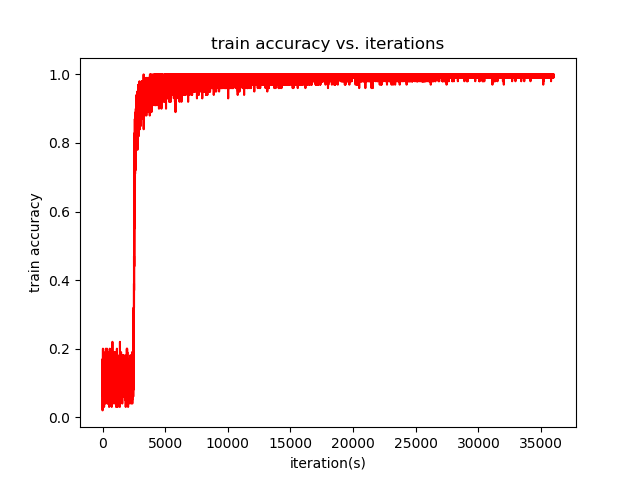
\includegraphics[width=\textwidth]{../results/trainacc2}
	\end{minipage}
	\caption{\label{trainres2}train loss curve and train accuracy curve in Experiments2}
\end{figure}

\begin{figure}[!h]
	\centering
	\begin{minipage}[t]{0.48\textwidth}
		\centering
		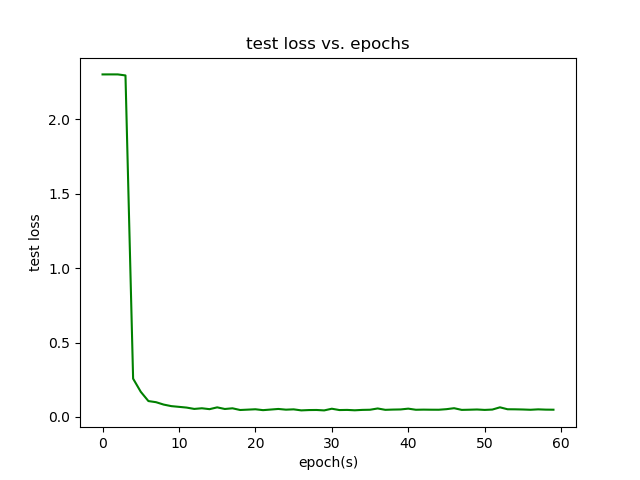
\includegraphics[width=\textwidth]{../results/testloss2}
	\end{minipage}
	\begin{minipage}[t]{0.48\textwidth}
		\centering
		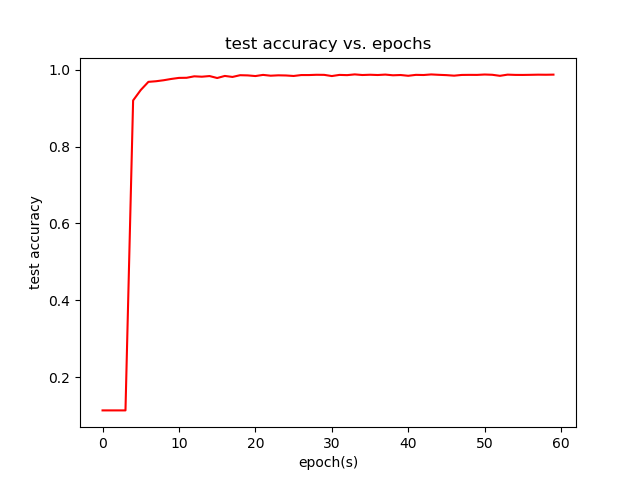
\includegraphics[width=\textwidth]{../results/testacc2}
	\end{minipage}
	\caption{\label{testres2}test loss curve and test accuracy curve in Experiments2}
\end{figure}
%\begin{table}[!ht]
%	\centering
%	\caption{\label{tab2}Network Structure with two hidden layers}
%	\begin{tabular}{|c|c|c|c|}
%		\hline
%		layer name & Input & Linear & Activation  \\
%		\hline
%		\multirow{2}{*}{Size} & \multirow{2}{*}{$784 \times 1$} & \multirow{2}{*}{$784 \times 128$} & Relu \\
%		& & & Sigmoid  \\
%		\hline
%		Linear & Activation & Linear &Loss \\
%		\hline
%		\multirow{2}{*}{$128\times 64$} &  Relu & \multirow{2}{*}{$64\times 10$} &EuclideanLoss \\
%		& Sigmoid & &SoftmaxCrossEntropyLoss \\
%		\hline 
%	\end{tabular}
%\end{table}

\section{Comparisions}
We summarize all test accuracys and test losses of every experiments and compare to the best experiment in the last homework as shown in Table \ref{tab3}. From the results we can get the following conclusions:
\begin{itemize}
	\item CNN has larger test accuracy than MLP, and from the experiments, we find that CNN has faster convergence speed than MLP. But CNN also has larger test loss than MLP. The reason may be that local interconnectivity of CNN results in losing some global information, but the information is not important for classification.
	\item Compare Experiment1 with Best experiment in HW1 we can find that CNN has less parameters than MLP with equal accuracy. And less parameters is not easy to result in overfitting. Therefore, CNN is much better than MLP in this task.
	\item For training time, MLP has less time than CNN in one epoch. The reason may be convolution operation has more time than Linear operation.
\end{itemize}

\begin{table}[!ht]
	\centering
	\caption{\label{tab3}Results Summary}
	\begin{tabular}{|c|c|c|c|}
		\hline
		Cases & Test Accuracy & Test Loss & Parameters Number\\
		\hline
		Experiment1 & 0.983 & 0.052 & 2143\\
		\hline
		Experiment2 & {\color{red} 0.987} & 0.048 & 203,628\\
		\hline
		Best experiment in HW1 & 0.983 & {\color{green} 0.021} & 109,187\\
		\hline
	\end{tabular}
\end{table}

\section{First convolution layer's output visualization}
Here we use the network in Experiment2 as shown in Figure \ref{fig2} to visualize the first convolution layer's output after ReLU for 0-9 digit images. We draw the output in each channel as shown in Figure \ref{visualization}

\begin{figure}[!h]
	\centering
	\begin{minipage}[t]{0.98\textwidth}
		\centering
		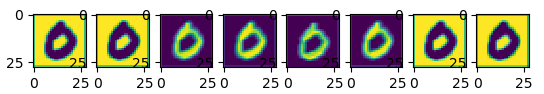
\includegraphics[width=\textwidth]{../results/00}
	\end{minipage}
	\begin{minipage}[t]{0.98\textwidth}
		\centering
		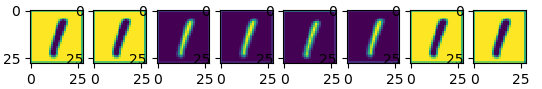
\includegraphics[width=\textwidth]{../results/01}
	\end{minipage}
	\begin{minipage}[t]{0.98\textwidth}
		\centering
		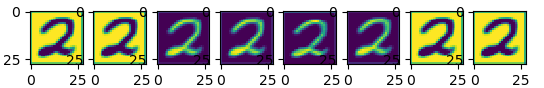
\includegraphics[width=\textwidth]{../results/02}
	\end{minipage}
	\begin{minipage}[t]{0.98\textwidth}
		\centering
		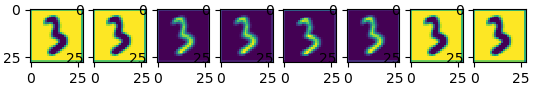
\includegraphics[width=\textwidth]{../results/03}
	\end{minipage}
	\begin{minipage}[t]{0.98\textwidth}
		\centering
		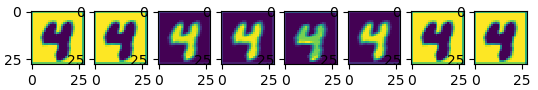
\includegraphics[width=\textwidth]{../results/04}
	\end{minipage}
	\begin{minipage}[t]{0.98\textwidth}
		\centering
		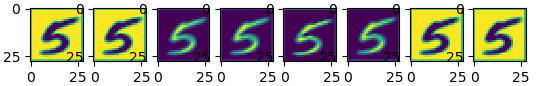
\includegraphics[width=\textwidth]{../results/05}
	\end{minipage}
	\begin{minipage}[t]{0.98\textwidth}
		\centering
		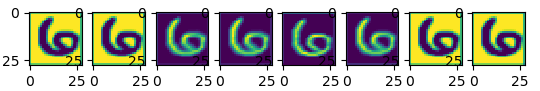
\includegraphics[width=\textwidth]{../results/06}
	\end{minipage}
	\begin{minipage}[t]{0.98\textwidth}
		\centering
		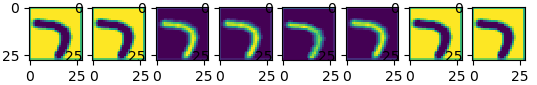
\includegraphics[width=\textwidth]{../results/07}
	\end{minipage}
	\begin{minipage}[t]{0.98\textwidth}
		\centering
		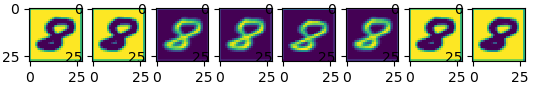
\includegraphics[width=\textwidth]{../results/08}
	\end{minipage}
	\begin{minipage}[t]{0.98\textwidth}
		\centering
		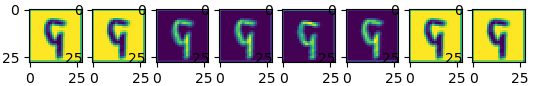
\includegraphics[width=\textwidth]{../results/09}
	\end{minipage}
	\caption{\label{visualization}The visualization of the first convolution layer's output after ReLU for 0-9 digit images in Experiments2 (8 channels)}
\end{figure}
\end{document}